\documentclass[12pt]{article}

\usepackage{tabto}
\usepackage[english]{babel}
\usepackage[utf8]{inputenc}
\usepackage{amsmath}
\usepackage{graphicx}
\usepackage[colorinlistoftodos]{todonotes}
\usepackage{float}
\restylefloat{figure}
\usepackage{subfig}

\usepackage[top=1.0in,bottom=1in,right=.5in,left=.5in,headheight=50pt,headsep=0.5cm]{geometry}
\usepackage{siunitx}
\usepackage{mcode}
\usepackage{url}
\usepackage{verbatim}
\usepackage{tipa}
\usepackage{fancyhdr}
\usepackage{enumerate}
\usepackage{color}
\definecolor{dkgreen}{rgb}{0,0.6,0}
\definecolor{gray}{rgb}{0.5,0.5,0.5}
\definecolor{mauve}{rgb}{0.58,0,0.82}
\lstset{frame=tb,
	language=R,
	aboveskip=3mm,
	belowskip=3mm,
	showstringspaces=false,
	columns=flexible,
	numbers=none,
	keywordstyle=\color{blue},
	numberstyle=\tiny\color{gray},
	commentstyle=\color{dkgreen},
	stringstyle=\color{mauve},
	breaklines=true,
	breakatwhitespace=false,
	tabsize=3,
	frame=single
}
\newcommand{\squeezeup}{\vspace{-5mm}}

\pagestyle{fancy}
\fancyhf{}
\rhead{Bruce Goldfeder}
\lhead{CSI 674 HW \#8}
\cfoot{Page \thepage}
\usepackage{sectsty}
\newcommand{\Rho}{\mathrm{P}}

\sectionfont{\fontsize{12}{15}\selectfont}

\subsectionfont{\fontsize{12}{15}\selectfont}

\title{CSI 674 Spring 2016 HW\#8}

\author{Bruce Goldfeder}

\date{\today}
\providecommand{\e}[1]{\ensuremath{\times 10^{#1}}}

\renewcommand{\thesubsection}{\thesection.\alph{subsection}}

\begin{document}
\maketitle
\NumTabs{12}

\begin{figure}[H]
\begin{flushleft}
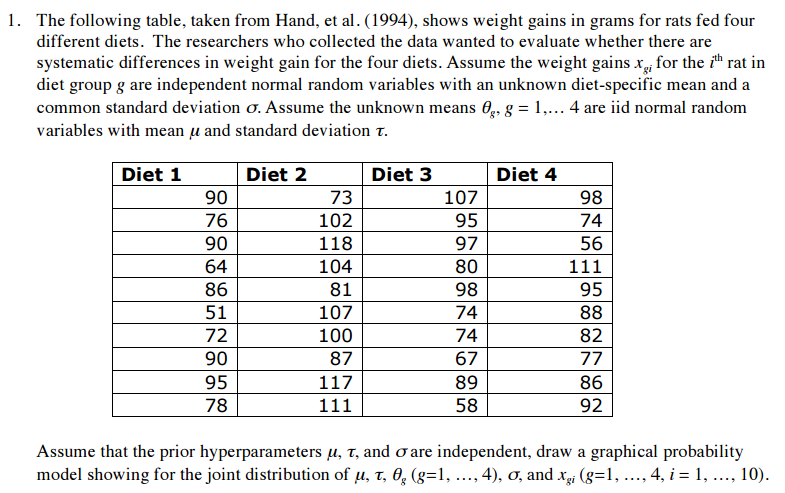
\includegraphics[scale=.9]{HW8Q1.png}
\end{flushleft}
\end{figure}
\squeezeup
\squeezeup
\squeezeup

\hspace{1cm} Given the assumptions of an unknown diet-specific mean and a common standard deviation I created the model below.  The model is normal / normal.


\begin{figure}[H]
\begin{flushleft}
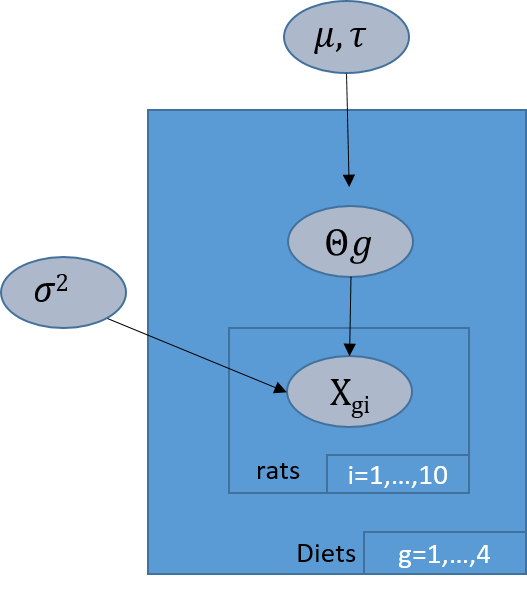
\includegraphics[scale=.9]{hierarchicalQ1d.png}
\end{flushleft}
\end{figure}


\begin{figure}[H]
\begin{flushleft}
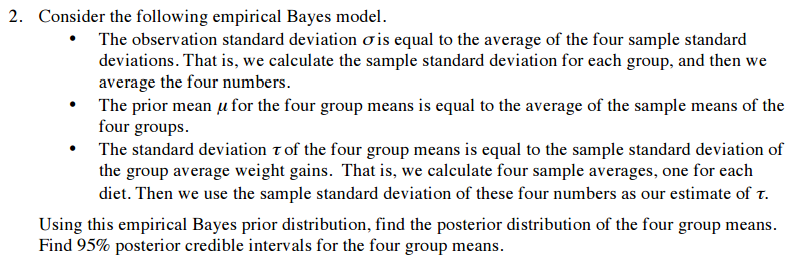
\includegraphics[scale=.9]{HW8Q2.png}
\end{flushleft}
\end{figure}
I ran the hierarchical bayes using the empirical bayes prior distribution using a loop over the sample values and updating $\mu$ and $\tau$ after each posterior is estimated.  The result was a N(87.25,2.28) with a 95\% credible interval of [82.77,91.73].  The following code was used to determine these values.
\lstinputlisting{HW8Q2.R}


\begin{figure}[H]
\begin{flushleft}
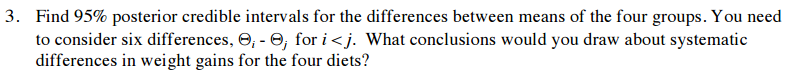
\includegraphics[scale=.9]{HW8Q3.png}
\end{flushleft}
\end{figure}
I added the following code to solve for the $\Theta_i$ - $\Theta_j$ where i>j.
\begin{verbatim}
diffs <- c(6)
labs <- c(6)

diff_n_labs <- data.frame(labs,diffs)

cnt = 1
for (i in 1:4) {
  for (j in 1:4) {
    if (i>j) {
      label <- paste(i,",",j)
      #print (label)
      diff_n_labs[cnt,1] <- label
      diff_n_labs[cnt,2] <- postThetas[i]-postThetas[j]
      cnt = cnt + 1
    }
  }
}
\end{verbatim}

This resulted in the following output:
\begin{verbatim}
> diff_n_labs
   labs      diffs
 2 , 1  8.3593657
 3 , 1  6.7083569
 3 , 2 -1.6510088
 4 , 1  6.2965797
 4 , 2 -2.0627861
 4 , 3 -0.4117772
\end{verbatim}
I plotted these below:
\begin{figure}[H]
\begin{flushleft}
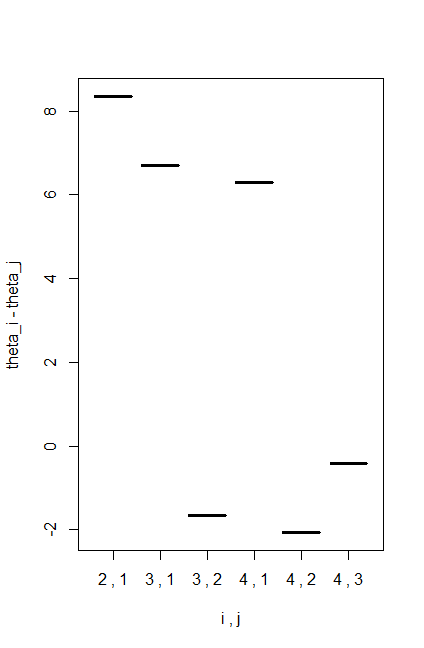
\includegraphics[scale=.9]{q3.png}
\end{flushleft}
\end{figure}
As expected the variance gets smaller and smaller until the difference is minimized for the fourth iteration minus the third.  This is consistent with the precision values which also get progressively smaller and the mean approaches the aggregate mean.
\begin{comment}

\begin{flushleft}
% QUESTION #4
4. Assume the $\mu,\tau,$ and $\sigma$ are independent; $\mu$ has an improper normal prior distribution with mean 0 and standard deviation $\infty$ (a uniform distribution); and $\tau$ and $\sigma$ have improper Gamma distributions with shape 0 and scale $\infty$.  Use Gibbs sampling to draw 10,000 samples from the joint posterior distribution on $\mu, \tau,$ and $\sigma$.\\
\medskip
\hspace{1cm}The answer to this question\\

\bigskip
% QUESTION #5
5. Do a tracelplot and plot the autocorrelation function of your samples.  On the basis of these plots, do you think it is necessary to discard a burn-in period?  Do you think you should do thinning?  Discuss.\\
\medskip
\hspace{1cm}The answer to this question\\


\bigskip
% QUESTION #6
6. Use your sample to evaluate whether there are differences in the four weight gains, and if so, the size of the difference.  Discuss.\\
\medskip
\hspace{1cm}The answer to this question


\end{flushleft}
\end{comment}

\end{document}